% PAGES: 
\chapter{Methodology and Project Organisation}
\label{mt:c:pm}

This chapter introduces development methods, tools and frameworks, which were used in this project. Furthermore, it shows the individual usage combinations of the 
presented methods and the project plan. Thereby, this plan presents the effective in comparison to the planned process of this project, visualised in a Gantt chart.

%Section_MDB describes the stengths of MDB etc.
\section{Software Development Process}
Mechatronic projects combine mechanical, electronic and software modules, which mostly are strongly related to each other. To solve problems of parallel development and a test driven architecture, the method \gls{MBD} is introduced and described here. This method is combined with the spiral model and builds an individual software development method for this project. The motivation thereby is to combine the strengths of a simulation driven \gls{MBD} with the advantageous evolutionary structure of the spiral model.

\subsection{Model Based Design}
\label{mt:c:pm:mbd}
\gls{MBD} is a popular method to encounter problems which come up in the development
of mechatronic products. These systems always involve mechanical, electrical, control
 and embedded components which are developed in different teams of
engineers with a specialised focus on one part of the complete project. Some of
these components are dependent on the results of other components before they can
be developed. This problem can be solved with \gls{MBD} and the
possibility to develop modules of the complete project by simulating their
environment, so the development can run highly parallel with the benefit that the
modules can be continuously tested in each phase of the project
\citeref[pp.1-2 Challenges of mechatronic product development]{EasLamTur09}.
Beside the direct challenges of mechatronic projects, problems also exist with the 
multiple domain modelling and development notations and languages. Legacy attempts
almost used several domain solutions and mapped these from the idea domain into the
solution domain. The problem in doing so is the additional effort to
spit up the problem in domain terms and to map the outcomes together. So another concept, which is adopted by
modern \gls{MBD} architectures is to create in a \gls{DSM} language, a model which is
generated to code from the domain-specific framework and to use the benefit to model the functionality and not indirect the code (See figure  \ref{fig:DSM.png}\footnote{This figure is derived from 
\citeref[p.13 Modelling functionality vs. modelling code]{SteKel09}})\citeref[pp.55-60 Chapter 3.3 Difference from other modelling approaches]
{SteKelJuhTol08}. One of the biggest disadvantages of \gls{MBD} architectures is that the
\gls{DSM} language is not as fine-grained and low-level as classic programming languages. \newpage This
can cause problems, especially in projects with very special requirements to the functionality which can not be
reflected without a workaround into the \gls{DSM} language. 

\begin{figure}[H]
	\centering
		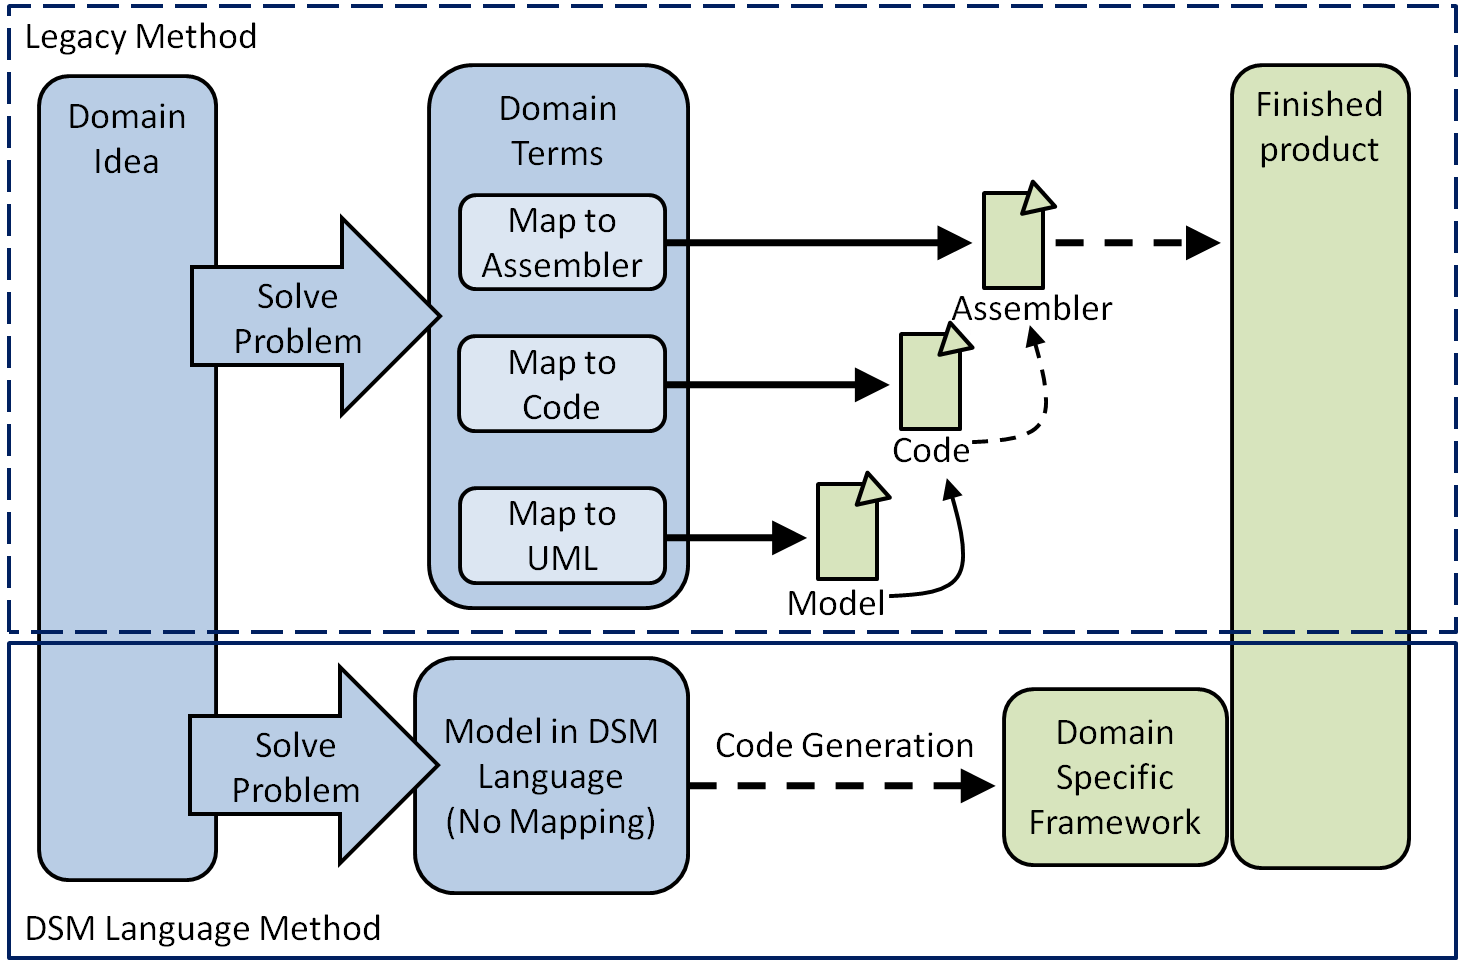
\includegraphics[width=1\textwidth]{graphic/DSM.png}
\caption{Legacy DSM vs. DSM Language approach}
	\label{fig:DSM.png}
\end{figure}

The development section in figure \ref{fig:SpiralModelAndMBD.png} includes the phases
and the corresponding key capabilities of \gls{MBD}. The first phase of \gls{MBD} is the
realisation of the researched and required components into a simulation
environment. Thereby physical components, environmental models and algorithms are
abstracted into systems by using domain-specific modelling tools with well
defined edges and intercommunication. The developed systems 
can be tested during the design phase simultaneously to analyse the system performance and correctness.
\newpage
Other key capabilities of \gls{MBD} are given in the implementation phase. Mostly, \gls{MBD}
tools allow to generate embedded code from the designed systems or to
combine handwritten code with the built simulation of the design phase. So the
implemented modules can be similarly tested in the adopted simulation
environment. Finally, components that have passed the tests at the implementation
phase can be integrated together. Ultimately, the final product can also be tested
with the \gls{MBD} tool by simulating the environment of the product, e.g. in a \gls{HIL}
test bench. \citeref[Model Based Design, MathWorks]{Mat10}

\subsection{Spiral Model}
\label{mt:c:pm:spiralModel}
Most of the \gls{UAV} stability and movement detection approaches were developed
iterative under consideration of the upcoming problems and obstacles 
\citebib[Iterative Development, Single and Dual Camera Feedback]
{AltOstMah02, AltOstTay03}
\citebib[Iterative Development, Landing and Position Control Development]
{LanSuePro08, LanSuePro09}. This procedure model will also be appropriate for this project, 
because the potential risks are difficult to identify. So the outcome of the development process has to be a
prototype that can be evaluated, tested and extended. A process model, which
provides an appropriate structure to face the iterative prototyping strategy
under consideration of the risk-aspects, is given with the spiral model. The
classic spiral model has typically four phases in which the product is
developed in an incremental evolutionary process. Derivates of this classic
model, for a customer evaluation focused on quality improvements, may have three,
five or six phases.
In the context of this project, the classic four phases
spiral model is used for scientific and feasibility studies and does not have to
provide further customer communication phases
\citeref[pp.36-38 The Spiral Model]{Pre01}.

\begin{figure}[H]
	\centering
		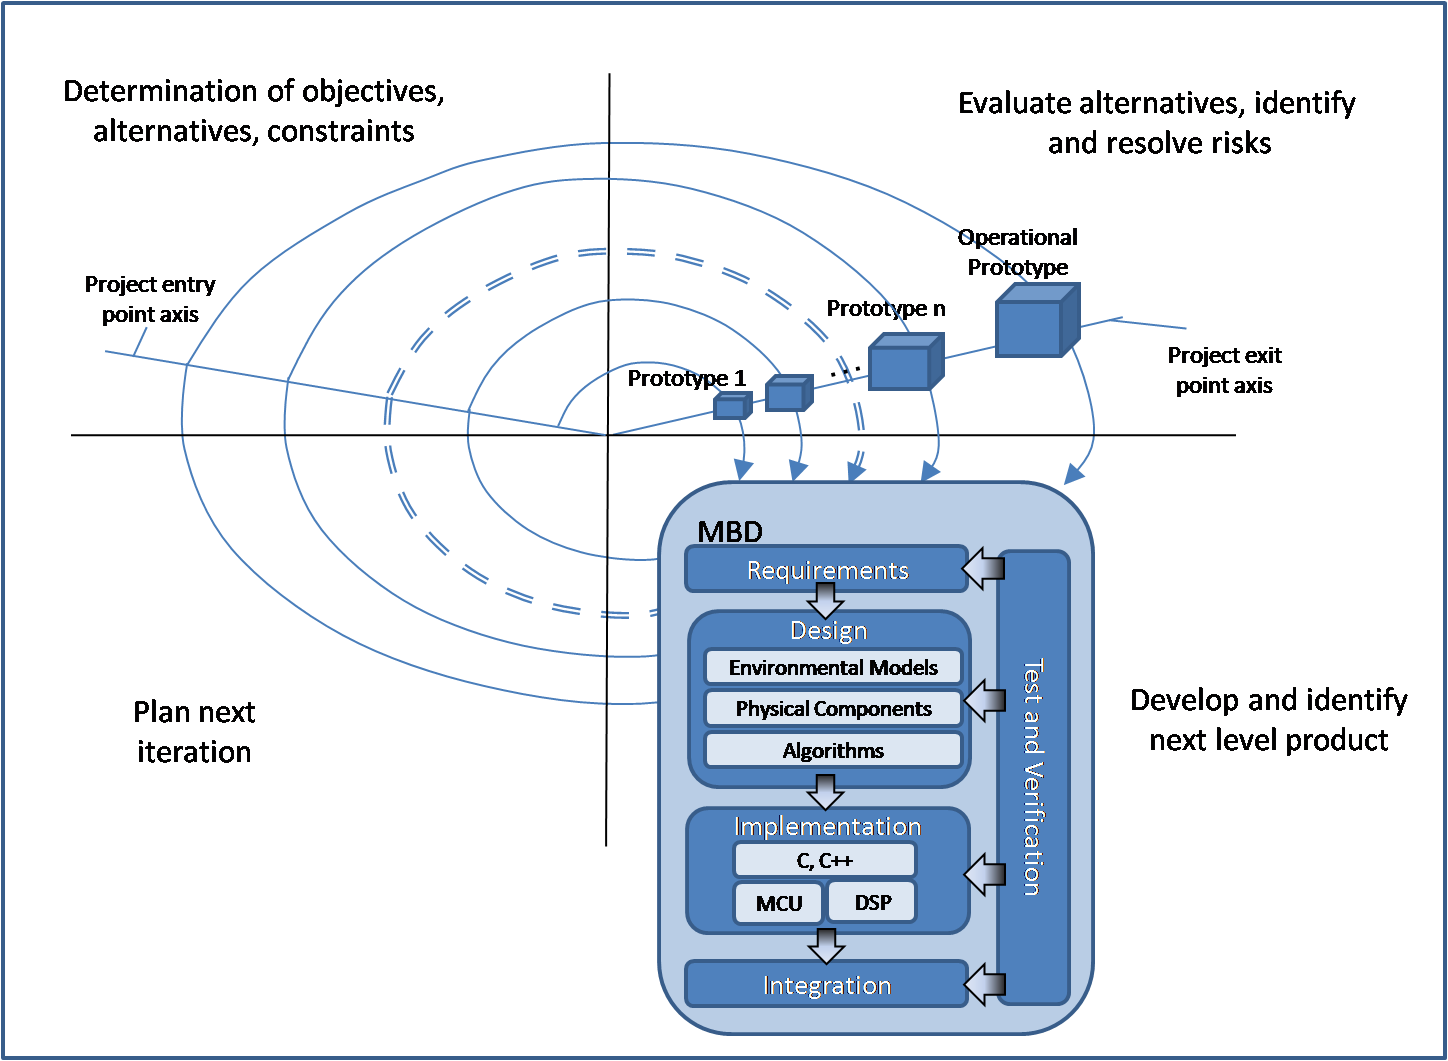
\includegraphics[width=1\textwidth]{graphic/SpiralModelAndMBD.png}
\caption{The Spiral Model in combination with Model Based Design}
\label{fig:SpiralModelAndMBD.png}
\end{figure}

A typical cycle of the four phases spiral model (\ref{fig:SpiralModelAndMBD.png})
 begins with the identification of
the objectives which have to be elaborated, like performance,
functionality, flexibility and so on. The next step is to evaluate the
alternatives in relation to the objectives and constraints, and to determine
significant sources of risks. After that, the next level
iteration of the product is planned. In the special case of this project, it is
advantageous to use \gls{MBD} in this phase by using the results of the previous phase as input.
This input can be a planned prototype, or requirements that describe the changes
to be executed. The output of the \gls{MBD} phase can be used again in the planning phase
for the next iteration \citeref
[pp.64-69 Spiral Model of the Software Process]{Boe88}.

\section{Tools and Architectures}
An overview of tools and architectures, which are analysed and used in the context of this project, is the main topic of this chapter. Thereby the detailed components of the presented architectures are examined with the focus of extensibility, exchangeability, modularity and so far. 

\subsection{MATLAB/Simulink}
\label{mt:c:pm:MATLABSimulink}
The software package \gls{MATLAB}\footnote{See \citebib[MATLAB] {Matlab11}}, developed by the company MathWorks \footnote{See \citebib[The MathWorks, Inc.] {MathWorks11}}, stands for solutions of high-performance numerical computation and visualisation.
Thereby \gls{MATLAB}'s main features and capabilities can be summarized in the groups visualized in figure \ref{fig:MATLAB-Simulink.png} \footnote{This figure is derived from the schematic diagram presented in \citeref[A schematic diagram of MATLAB'S main features]{Rud06}}.
\gls{MATLAB}'s built-in functions provide tools for linear algebra computations, data analysis, signal processing, optimisation, numerical solution of \gls{ODE} and further types of scientific computation. For visualisation, \gls{MATLAB} supports numerous graphic functions for 2-D and 3-D graphics and animations. Modules programmed in C/C++ or Fortran can be integrated into \gls{MATLAB} by using the external interface using the Mex-files. This facility allows to simulate the environment of an embedded algorithm and to test it, to include legacy modules of previous developments or libraries which are programmed in the supported languages. 
\newpage
\gls{MATLAB} also provides an own \gls{4GL}(also denoted as \gls{MATLAB}) \gls{DSM} language for programming focused on the fast development of functions or applications. Various toolboxes of \gls{MATLAB} allow the development of special applications such as symbolic computations, image processing, statistics etc. and reflect the idea of \gls{DSM}. The list of toolboxes keeps growing over time and releases of \gls{MATLAB} \citeref[p.3 What is MATLAB?]{Rud06}.
Beside the programming interface of \gls{MATLAB}, Simulink provides an environment for multi-domain simulation and \gls{MBD} of dynamic embedded systems. This graphical interface also provide easy access to the complete \gls{MATLAB} continuum of tools \footnote{See \citebib[Simulink]{Simulink11}}. 

\begin{figure}[H]
	\centering
		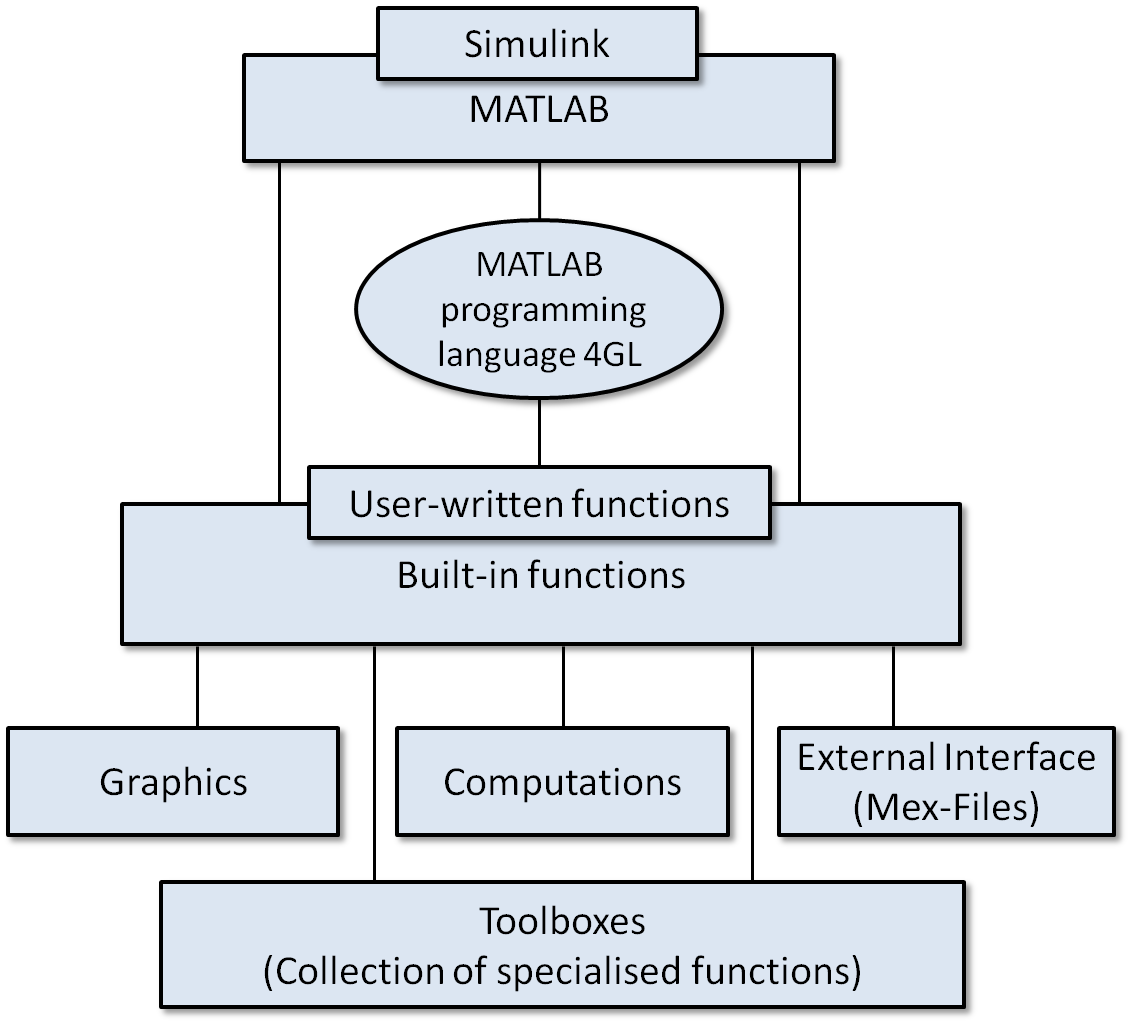
\includegraphics[width=0.9\textwidth]{graphic/MATLAB-Simulink.png}
\caption{MATLAB/Simulink's schematic diagram of main features}
	\label{fig:MATLAB-Simulink.png}
\end{figure}


\subsection{OpenCV}
\label{mt:c:pm:openCV}
\gls{OpenCV}\footnote{See \citebib{OpenCV2_0}} is one of the most popular open source computer vision libraries for scientific and industrial projects. It contains over 500 functions that span many areas in computer vision such as medical imaging, factory product inspection, security, camera calibration, stereo vision, robotics and so on. The main components of \gls{OpenCV} are visualized in figure \ref{fig:OpenCV.png} \footnote{This basic structure overview bases on the figure presented in \citeref[p.33 Chapter 1, The basic structure of OpenCV]{GarKae08}}. The component \gls{CV} contains the basic image processing and higher-level computer vision algorithms. Another important part strongly related to computer vision is the machine learning ability. So \gls{OpenCV} provides statistic classifier and clustering tools which allow this ability in the \gls{MLL} component. \gls{OpenCV}'s \gls{I_O} component \gls{HighGUI} contains functions and routines for fast loading and storing of image or video data and a \gls{GUI}. Finally, the core data structures and algorithms are located in the component CXCORE which supports data transforms, matrix algebra, object persistence, memory management, error handling and further core capabilities \citeref[pp.1-33 Chapter 1, Overview]{GarKae08}.

\begin{figure}[H]
	\centering
		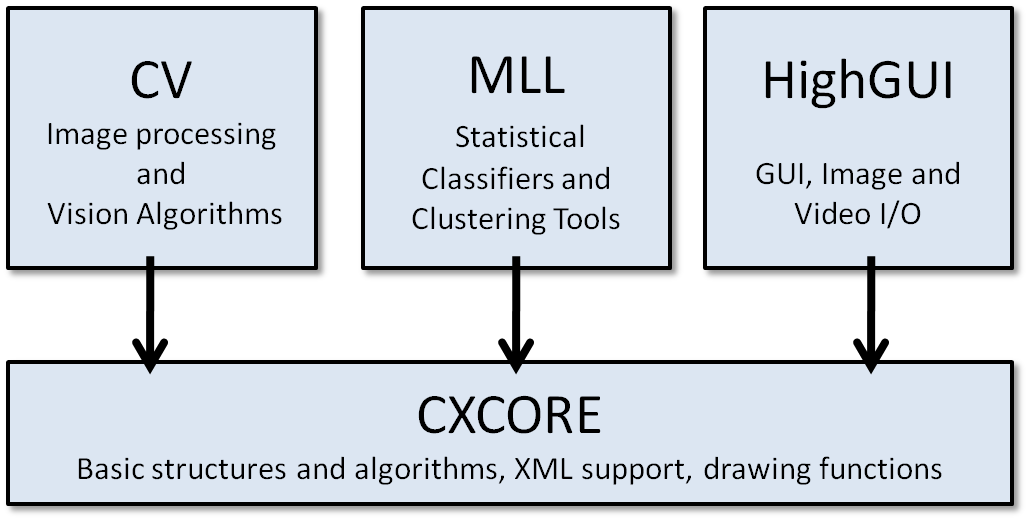
\includegraphics[width=1\textwidth]{graphic/OpenCV.png}
\caption{OpenCV's basic structure}
	\label{fig:OpenCV.png}
\end{figure}

\section{Strengths and Risks}
\label{mt:c:pm:Strengths and Risks}
As mentioned in chapter \ref{mt:c:pm:mbd}, the strengths of \gls{MBD} are the possibility of parallel development of mechatronic, electrical or software components, and the test facility during each phase that is presented in the \gls{MBD} process in \ref{fig:SpiralModelAndMBD.png}. Beside this advantages, \gls{MBD} bases on the strategy to create simulations of components and to refine these from an abstract level to a more detailed level and finally to the real execution environment. Thereby, this way of development can include risks which can lead, at the worst, to a restart of the project development. As presented in the spiral process model, risks should be analysed and classified in a previous phase before development. Related to the simulation development of this project, the most important risks are analysed in \ref{fig:Risks}\footnote{Related risk preventions and provisions are shown in 
\ref{mt:c:expResults:ReproducibilityReliability}, 
\ref{mt:c:design:Simulation of Embedded System Quadrocopter}, \ref{mt:c:design:Analysis of Existing Quadrocopter Architecture}, 
\ref{mt:c:design:Optical Movement Detection Architectures}}.
\newpage
The analysis thereby includes the identified risk, the effect, which can raise if the risk becomes real, the classification of the risk related to the seriousness, and the strategy which should be executed if the risk occurs or to prevent the risk. The corresponding risk preventions in this work are presented with references to the corresponding chapters. Furthermore, the classification shows if the risk is ignorable, threatens to delay the project could even lead to a catastrophic project fail.


\begin{figure}[H]
	\centering
		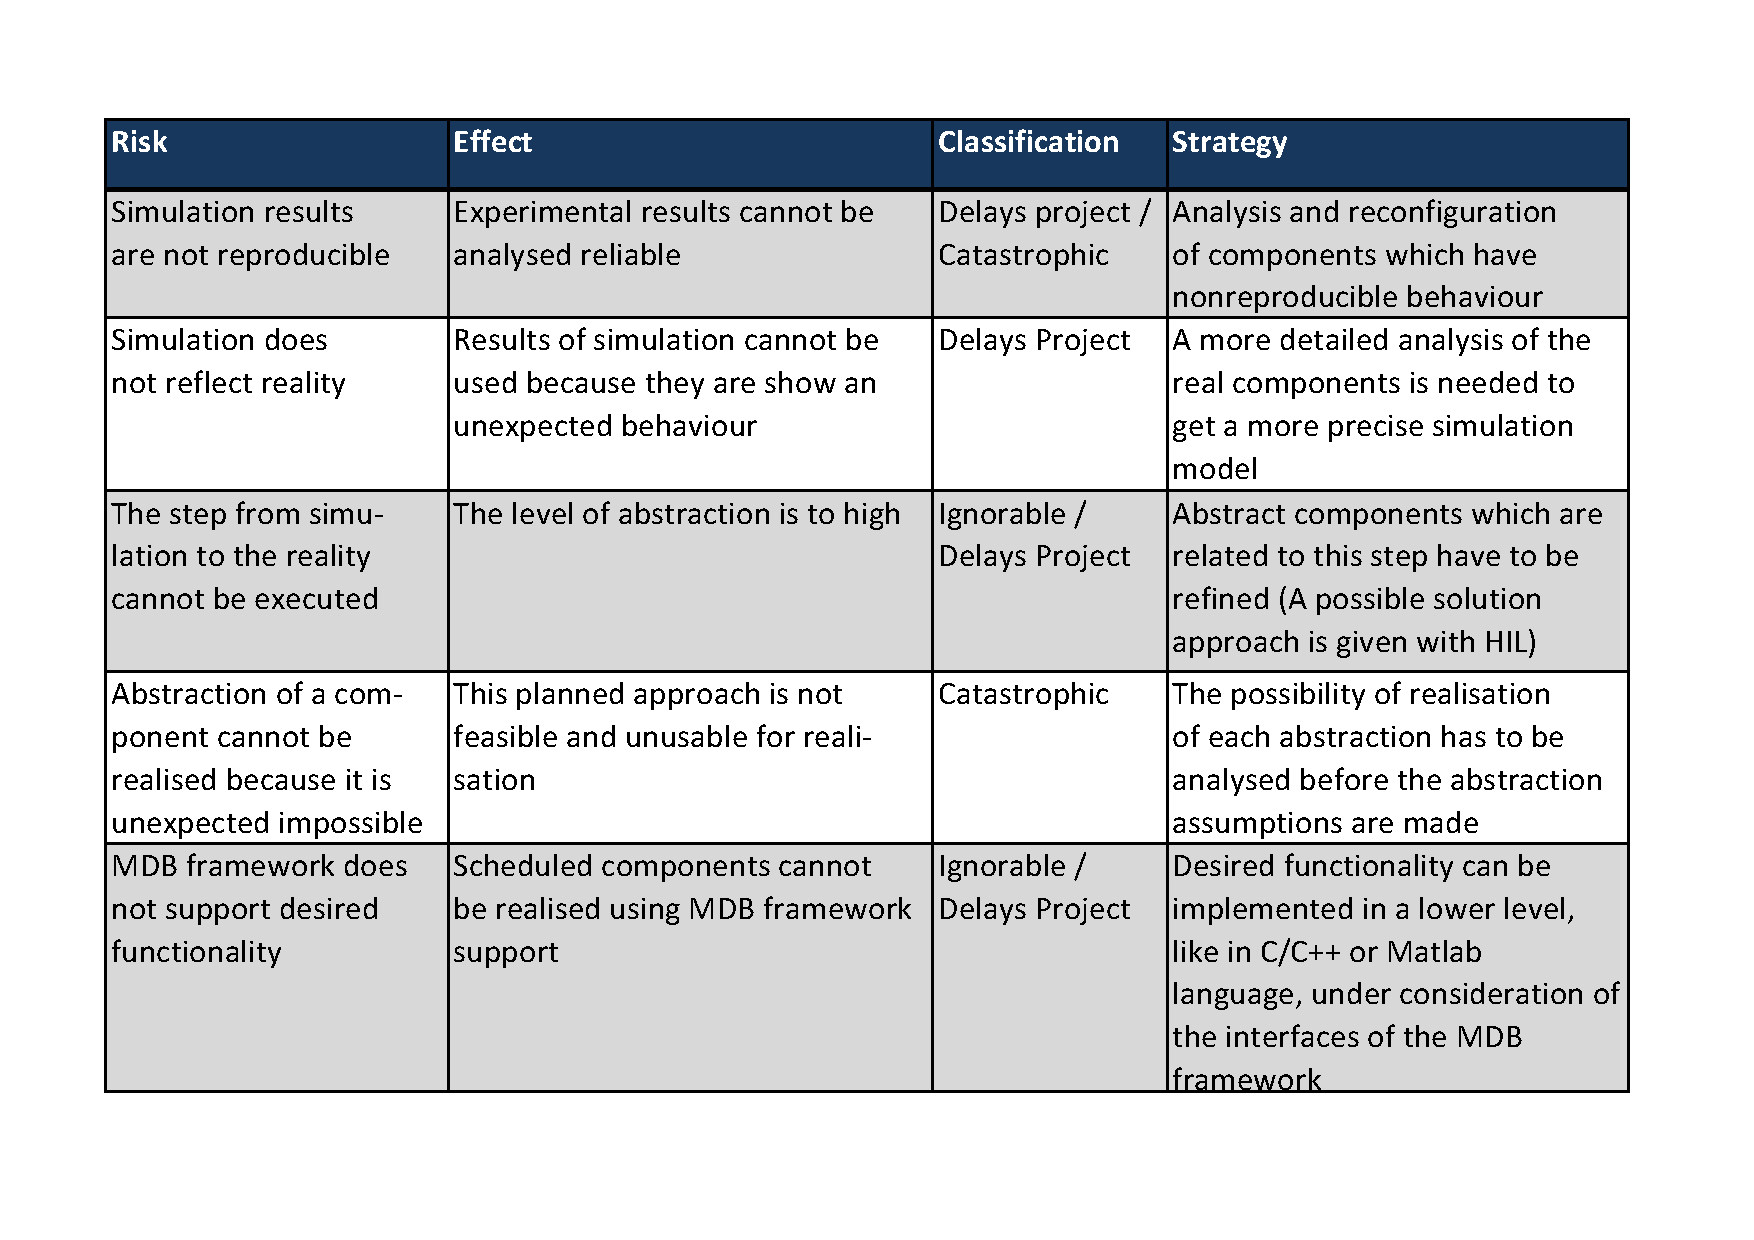
\includegraphics[width=1\textwidth]{graphic/RiksAnalysisTable.pdf}
\caption{Possible risks, effect, classification and solution strategy}
\label{fig:Risks}
\end{figure}
%
%\begin{table}
%\begin{tabular}{|p{3.2cm}|p{3.2cm}|p{3.2cm}|p{3.2cm}|}
%\hline
 %Risk & Effect & Classification & Strategy\\
%\hline
%\hline
 %Simulation results are not reproducible &
 %Experimental results cannot be analysed reliable &
 %Delays project / Catastrophic &
 %Analysis and reconfiguration of components which have non-reproducible behaviour \footnote{See chapter 
%\ref{mt:c:expResults:ReproducibilityReliability}} (See chapter )\\
%%\ref{mt:c:expResults:ReproducibilityReliability}
%\hline
 %Simulation does not reflect reality &
 %Results of simulation cannot be used because they are show an unexpected behaviour & 
 %Delays Project &
 %A more detailed analysis of the real components is needed to get a more precise simulation model (See chapter )\\% \ref{mt:c:expResults:AnalysisofImageProcessing:LimitsofSimulationenvironment}

%\hline
 %The step from simulation to reality cannot be executed &
 %The level of abstraction is to high &
 %Ignorable / Delays Project &
 %Abstract components which are related to this step have to be refined (A possible solution approach is presented with HIL in 
%)\\%\ref{mt:c:design:Simulation of Embedded System Quadrocopter}

%\hline
%Abstraction of a component cannot be realised because it is unexpected impossible &
%This planned approach is not feasible and unusable for realisation &
%Catastrophic &
%The possibility of realisation of each abstraction has to be analysed before the abstraction assumptions are made (See chapter )\\%\ref{mt:c:design:Analysis of Existing Quadrocopter Architecture}

%\hline
%MDB framework does not support desired functionality &
%Scheduled components cannot be realised using MDB framework support &
%Ignorable / Delays Project &
%Desired functionality can be implemented in a lower level like in C/C++ or Matlab language, under consideration of the interfaces of the MDB framework (A sample for this strategy is presented in )\\%\ref{mt:c:design:Optical Movement Detection Architectures}

%\hline
%\end{tabular}
%\caption{Possible risks, their effect, their classification and their solution strategy}
%\label{fig:Risks}
%\end{table}

%1.Risks of DSM and MDB -> not to find specific solution component for 
%specific problem
%2.Strength of DSM and MDB Abstraction -> Concretisation Sehe Tagebuch Eintrag 01.02.2011
%Auf dieses Kapitel und speziell auf 2. wird in Problems, Limitations and Assumptions referenziert!!!

%ERW�HNE als Risk, das thema was auch mit Prof. Friedrich diskutiert wurde. Simulationsabstraktion ist gut, aber es kann einen
% entscheidenden punkt abstrahieren welcher nach der wiss. Untersuchung zeit das alles um sonst war weil es wegen diesen Punkt nicht geht. Das 
% ist der gr�sste Risk des Projektes, deswegen diskutiere �ber die Abstraktionen in  2. Problems, Limitations and Assumptions ob es annahmen 
% die sp�ter zu einem GAU Punkt f�hren k�nnen, bewerte das risiko und bespreche risk-strategien

\newpage
\section{Project Management}

Based on the spiral model presented in \ref{mt:c:pm:spiralModel}, the project plan executed in this Master's Thesis project includes one circle of all phases and ends with the release of the first prototype and the corresponding research and documentation. The Gantt chart, shown in figure \ref{fig:ProjectPlan.pdf}, visualises the original planned and the truly executed project plan 
\footnote{The original planned tasks/milestones are grey/white and the truly executed are red/blue/black}. Regarding the first few tasks of analysis and research of relevant topics, the time resources were guessed quite good because the time-drift between the issues adds up to only few days. After the second milestone, which symbolises the start of the \gls{MBD} phase, the time miscalculation increases dramatically. 

A reason for that could be the missing practical experience and the necessity to gain new knowledge of architectures and tool-kits of the \gls{MBD} tool which were not expected before. This experience shows that more time has to be planned in the context of a project like this, to research which components should be used and to get familiar with these. Furthermore, it is interesting to see that the parallel tasks, which include two parallel lines for documentation and parallel research, could be executed as planned for the interim report and final dissertation. 

The characteristic not expected of these parallel tasks was the fact that the modelling and research parallel to the documentation took nearly the same time. A reason for that is the fact that the research results show mostly unexpected phenomenons which were examined more closely to find out the reasons for these effects.
\newpage
Another reason of delay was the expectation that most of the needed components could only be designed with the \gls{MBD} tool, and the execution code of the simulation can be generated automatically.
But some of the needed functions were not supported by the framework, which lead to the necessity to implement the components manually. Overall, the expected critical path 
(red) was correct, because the documentation of the dissertation claimed the biggest time resources and delays. This could base on the fact that the complex parts of this dissertation are difficult to be presented and reduced so the reader has the chance to understand the presented material.

\begin{figure}[H]
	\centering
		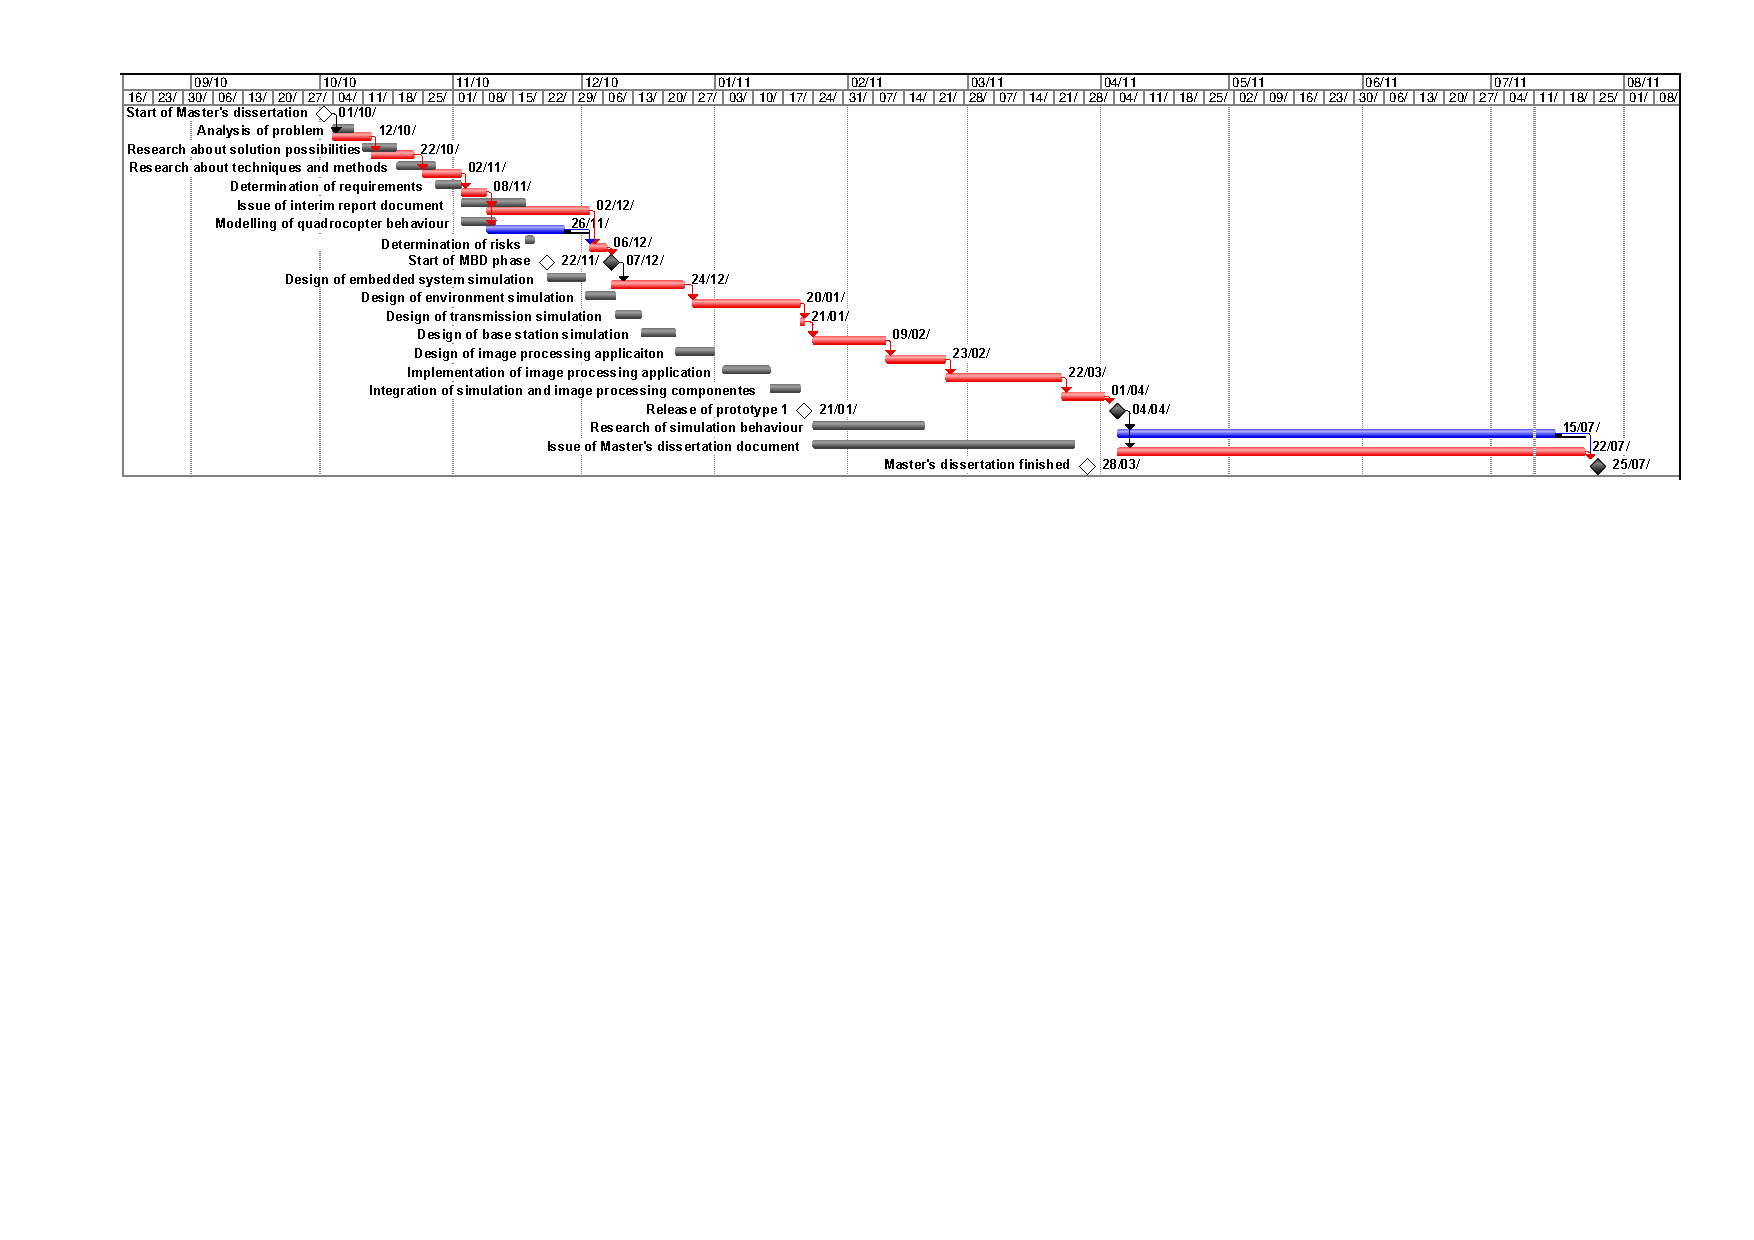
\includegraphics[width=1\textwidth, height=0.4\textwidth]{graphic/ProjectPlan.pdf}
\caption{Executed project plan with time drifts (Gantt Chart)}
	\label{fig:ProjectPlan.pdf}
\end{figure}